\documentclass[aspectratio=169]{beamer}

\usepackage[ngerman]{babel}
\usepackage[utf8]{inputenc}
\usepackage[T1]{fontenc}
\usepackage{helvet}
\usepackage{pifont}
\usepackage{lipsum}
\usepackage{graphicx}
\usepackage{makecell}
\usepackage{array}

\usepackage{customStyle}

\setbeamertemplate{navigation symbols}{}
\setbeamercovered{transparent}
\setbeamerfont{default}{size=\small}
\AtBeginDocument{\usebeamerfont{default}}

\title{CI/CD Rollouts auf Rancher mit Terraform}
\subtitle{Fraunhofer DevOps Day 2024}
\author{Niklas Letz}
\institute{DevOps Engineer @ ventx GmbH}
\date{\small 13. August 2024}


\begin{document}

\begin{frame}
    \vspace{.2cm}
    \titlepage
    \vspace{-.6cm}
    \begin{figure}[htbp]
        \centering
        
\includegraphics[width=.5\textwidth]{img/logo_ventx.png}
    \end{figure}
\end{frame}

\begin{frame}
    \tableofcontents[sectionstyle=show,
    subsectionstyle=show/shaded/hide,
    subsubsectionstyle=show/shaded/hide]
\end{frame}

\section{Über mich}
\begin{frame}{Über mich}
    \begin{columns}
        \column{.6\textwidth}
            \centering
            \begin{itemize}
                \item Vor 25 Jahren in München geboren\pause
                \item Seit April 2021 DevOps Engineer bei der ventx GmbH\pause
                \item Wir helfen unseren Kunden dabei, ihre Infrastruktur zu optimieren und fit für die Zukunft zu machen und dadurch Kosten zu optimieren\pause
                \item Mehrfach Kubernetes zertifiziert\pause
                \item Seit März als Externer für die Fraunhofer Zentralverwaltung tätig\pause
                \item Dort zuständig für die Entwicklung einer maßgeschneiderten On-Demand Kubernetes Lösung basierend auf Rancher
            \end{itemize}
        \column{.4\textwidth}
            \begin{figure}[htbp]
                \centering
                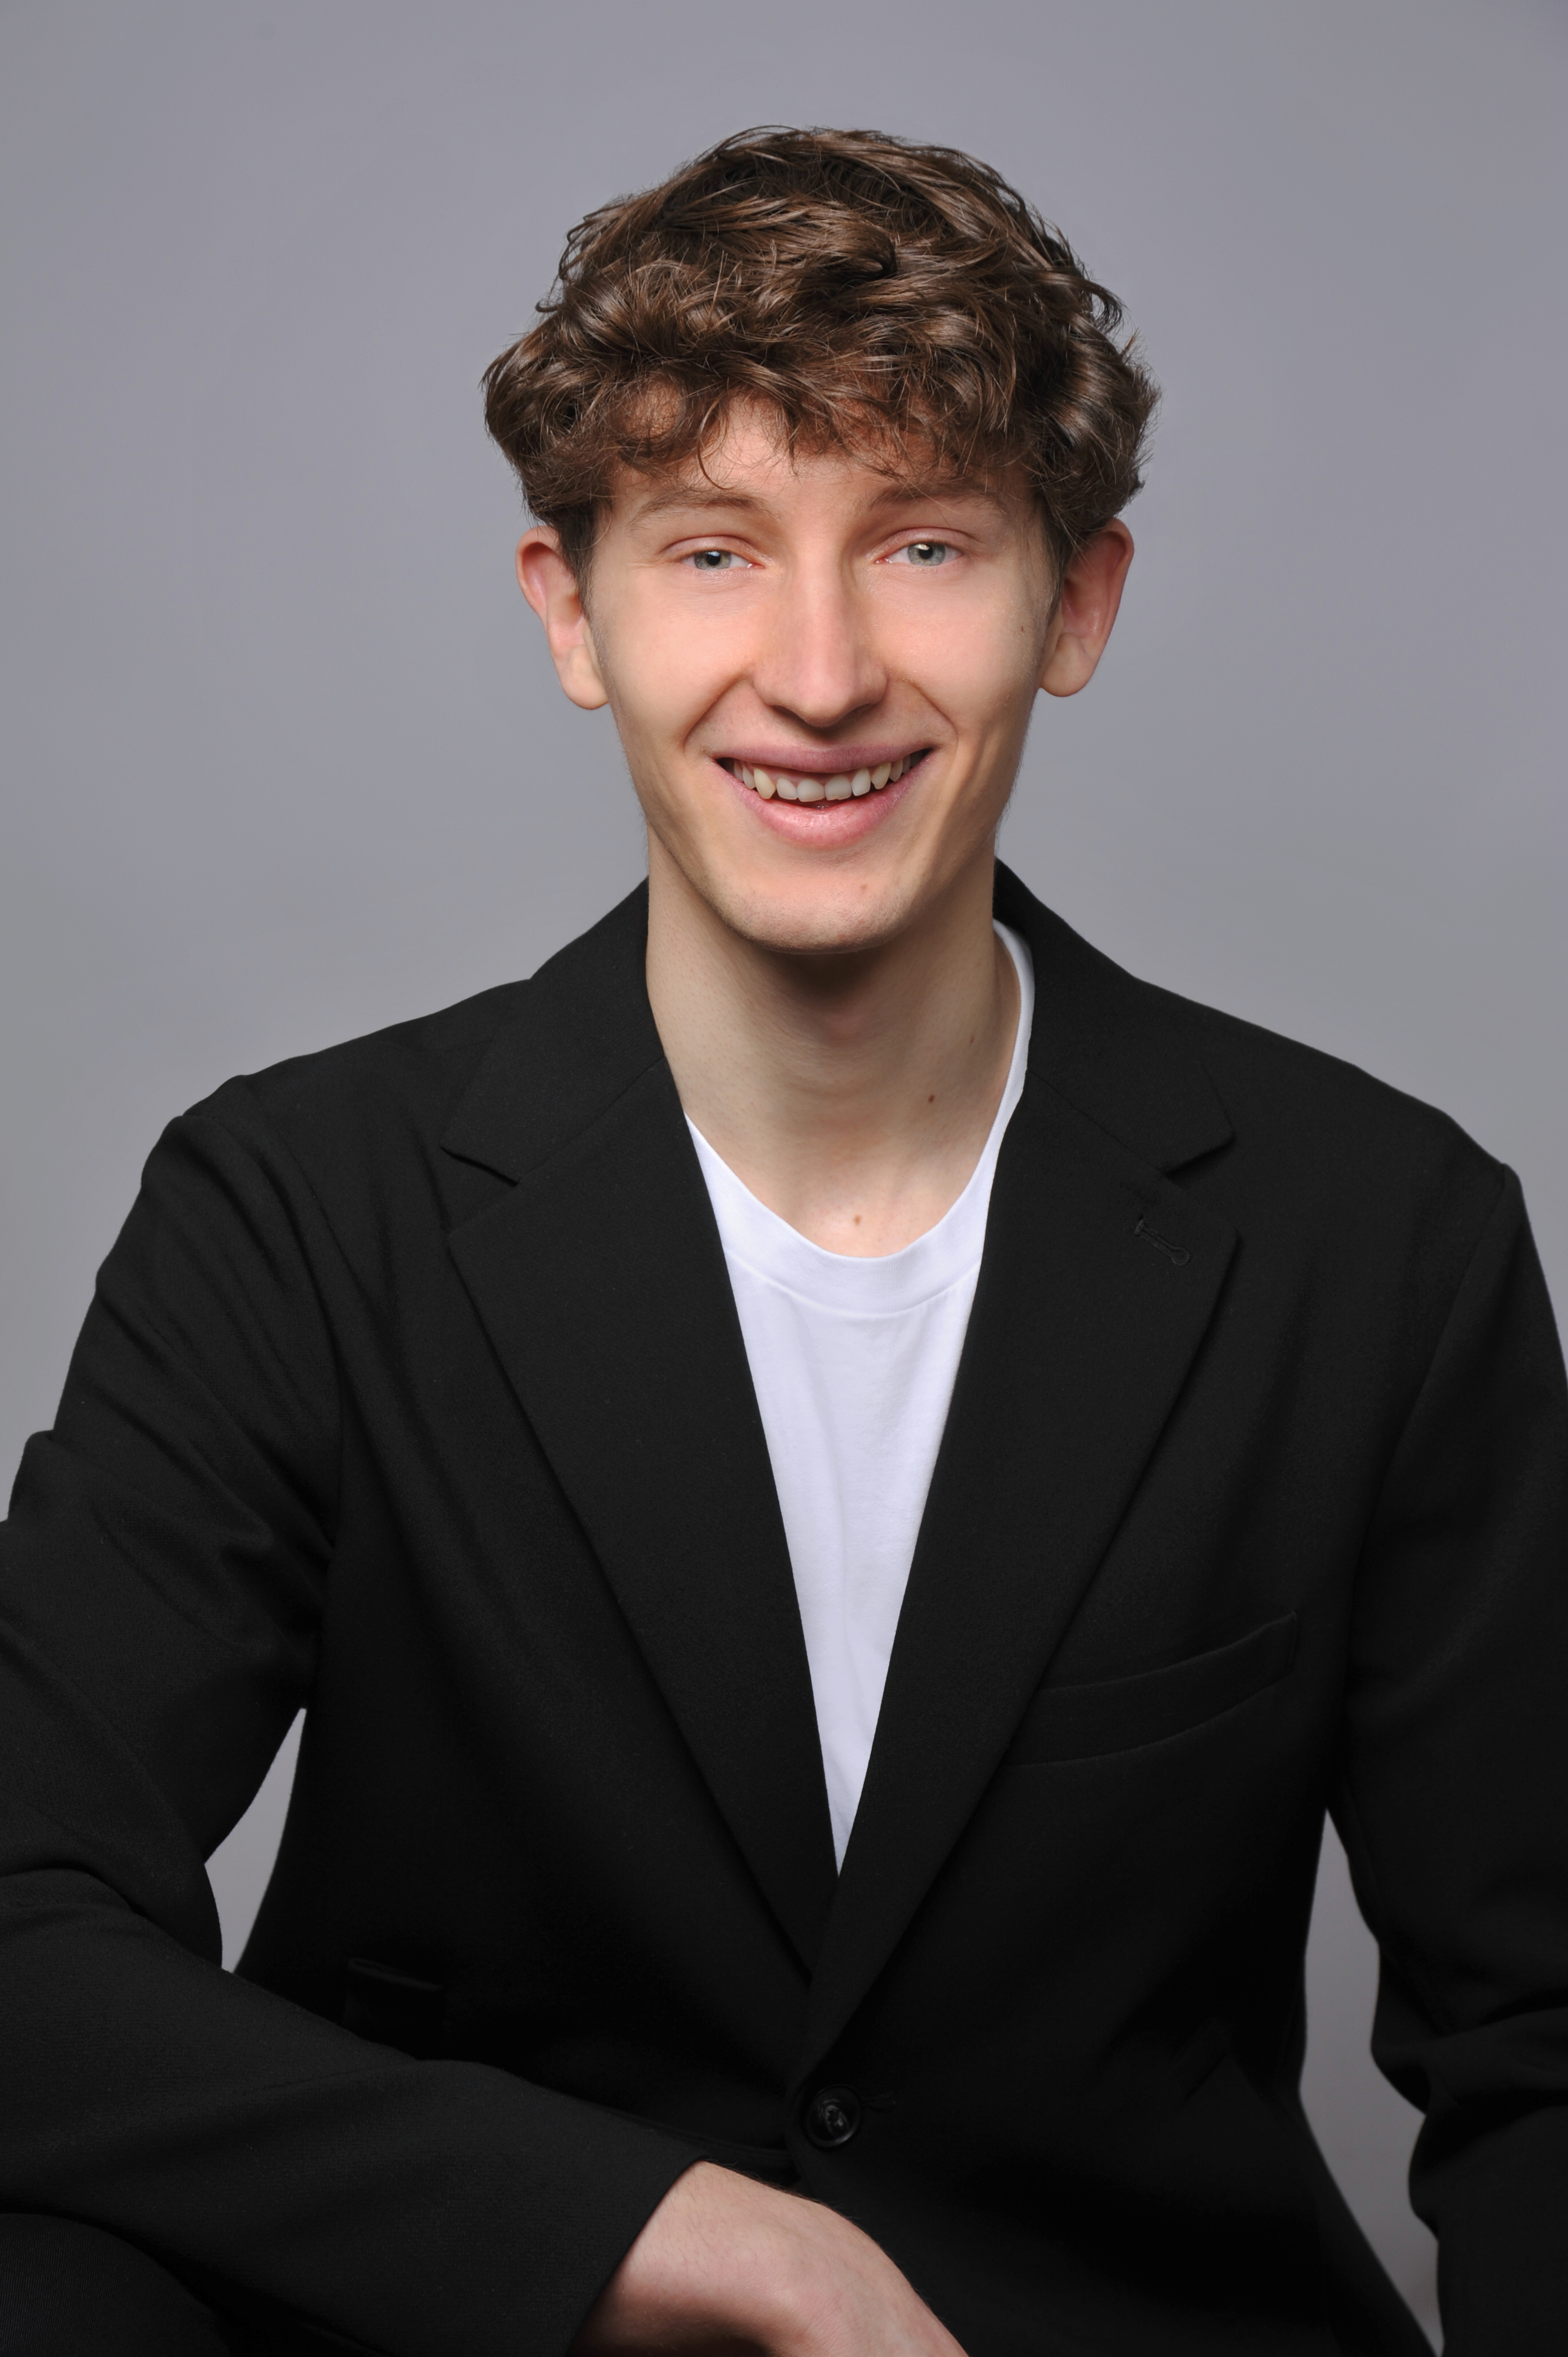
\includegraphics[width=.7\textwidth]{img/profile.jpg}
            \end{figure}
    \end{columns}
\end{frame}
\section{Einleitung}
\begin{frame}{Einleitung}
    \begin{itemize}
        \item Mit "`einem Klick"' einen voll funktionsfähigen Kubernetes Cluster bereitstellen\pause
        \item Das innerhalb weniger Minuten\pause
        \item On-Demand, je nach Bedarf\pause
        \item Einfach an die individuellen Bedürfnisse anpassbar\pause
        \item Ermöglicht durch das Zusammenspiel mehrerer DevOps Tools\pause
        \item Nach den Best-Practice Prinzipien\pause
        \item In Zusammenarbeit mit Sascha Weiland und Tamara Muryshkin
    \end{itemize}
\end{frame}

\subsection{Techstack}
\begin{frame}{Techstack}
    \renewcommand{\arraystretch}{2}
    \begin{table}[htbp]
        \centering
        \begin{tabular}{l@{\hskip 1.25cm}l}
            \textbf{Technologie} & \textbf{Einsatz} \\
            \hline
            GitLab CI/CD & \makecell[l]{Bereitstellen einer GitLab CI/CD Komponente \\ als Template für den Rollout-Prozess} \\
            \hline
            Terraform & \makecell[l]{Infrastructure-as-Code Modul \\ für die Cluster-Provisionierung auf Rancher} \\
            \hline
            Argo CD & \makecell[l]{GitOps Tool für das automatische \\ Bootstrapping des Clusters mit Standard Apps} \\
            \hline
            Rancher & \makecell[l]{Kubernetes Management Platform \\ für die sogenannten Rancher Downstream Cluster} \\
        \end{tabular}
    \end{table}
\end{frame}

\subsection{Was ist Rancher?}
\begin{frame}{Was ist Rancher?}
    \begin{itemize}
        \item Eine Kubernetes Cluster Orchestrierungs-Platform von SUSE\pause
        \item Managen von vielen Kubernetes Clustern auf einmal\pause
        \item Bereitstellen von Kubernetes-as-a-Service\pause
        \item 100\% open source\pause
        \item Unterstützt mehrere Platformen\pause
            \begin{itemize}
                \item AWS\pause
                \item Azure\pause
                \item Google Cloud Platform\pause
                \item VMware
            \end{itemize}\pause
        \item Rancher spricht mit APIs der Infrastruktur-Provider\pause
        \item Bekannteste Alternative = Red Hat OpenShift
    \end{itemize}
\end{frame}

\section{Architektur}
\begin{frame}{Architekturdiagramm}
    \begin{columns}
        \column{.6\textwidth}
            \begin{figure}[htbp]
                \centering
                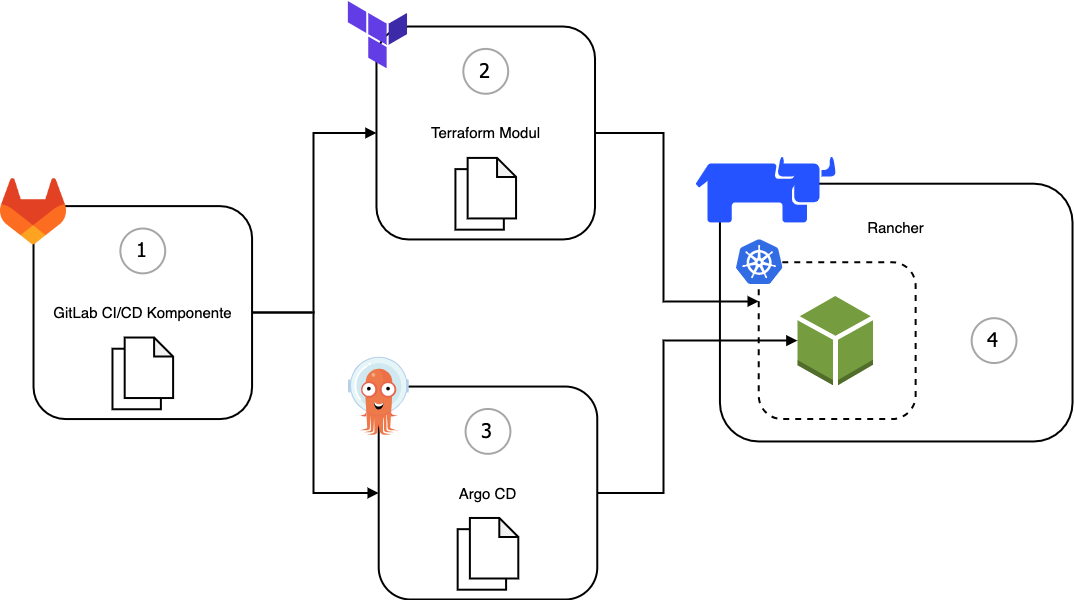
\includegraphics[width=1\textwidth]{img/chart_drawio.png}
            \end{figure}
        \column{.4\textwidth}
            \centering
            \footnotesize
            \begin{itemize}
                \item[\ding{172}] Die GitLab Pipeline authentifiziert, validiert und deployt alle involvierten Bausteine
                \pause
                \item[\ding{173}] Das Terraform Modul umfasst das eigentliche Deployment des Rancher Clusters sowie einiger Abhängigkeiten
                \pause
                \item[\ding{174}] Argo CD kümmert sich darum, den Cluster mit notwendigen Apps und Settings zu bootstrappen
                \pause
                \item[\ding{175}] Man erhält einen von Rancher orchestrierten Kubernetes Cluster (a.k.a. Downstream Cluster)
            \end{itemize}
    \end{columns}
\end{frame}

\section{Live Demo}
\begin{frame}
    \centering\huge Live Demo
\end{frame}

\section{Q \& A}
\begin{frame}
    \centering\huge Vielen Dank! :-)
\end{frame}

\begin{frame}
    \centering\huge Fragen?
\end{frame}

\end{document}
